\begin{figure}[t]
  \centering
  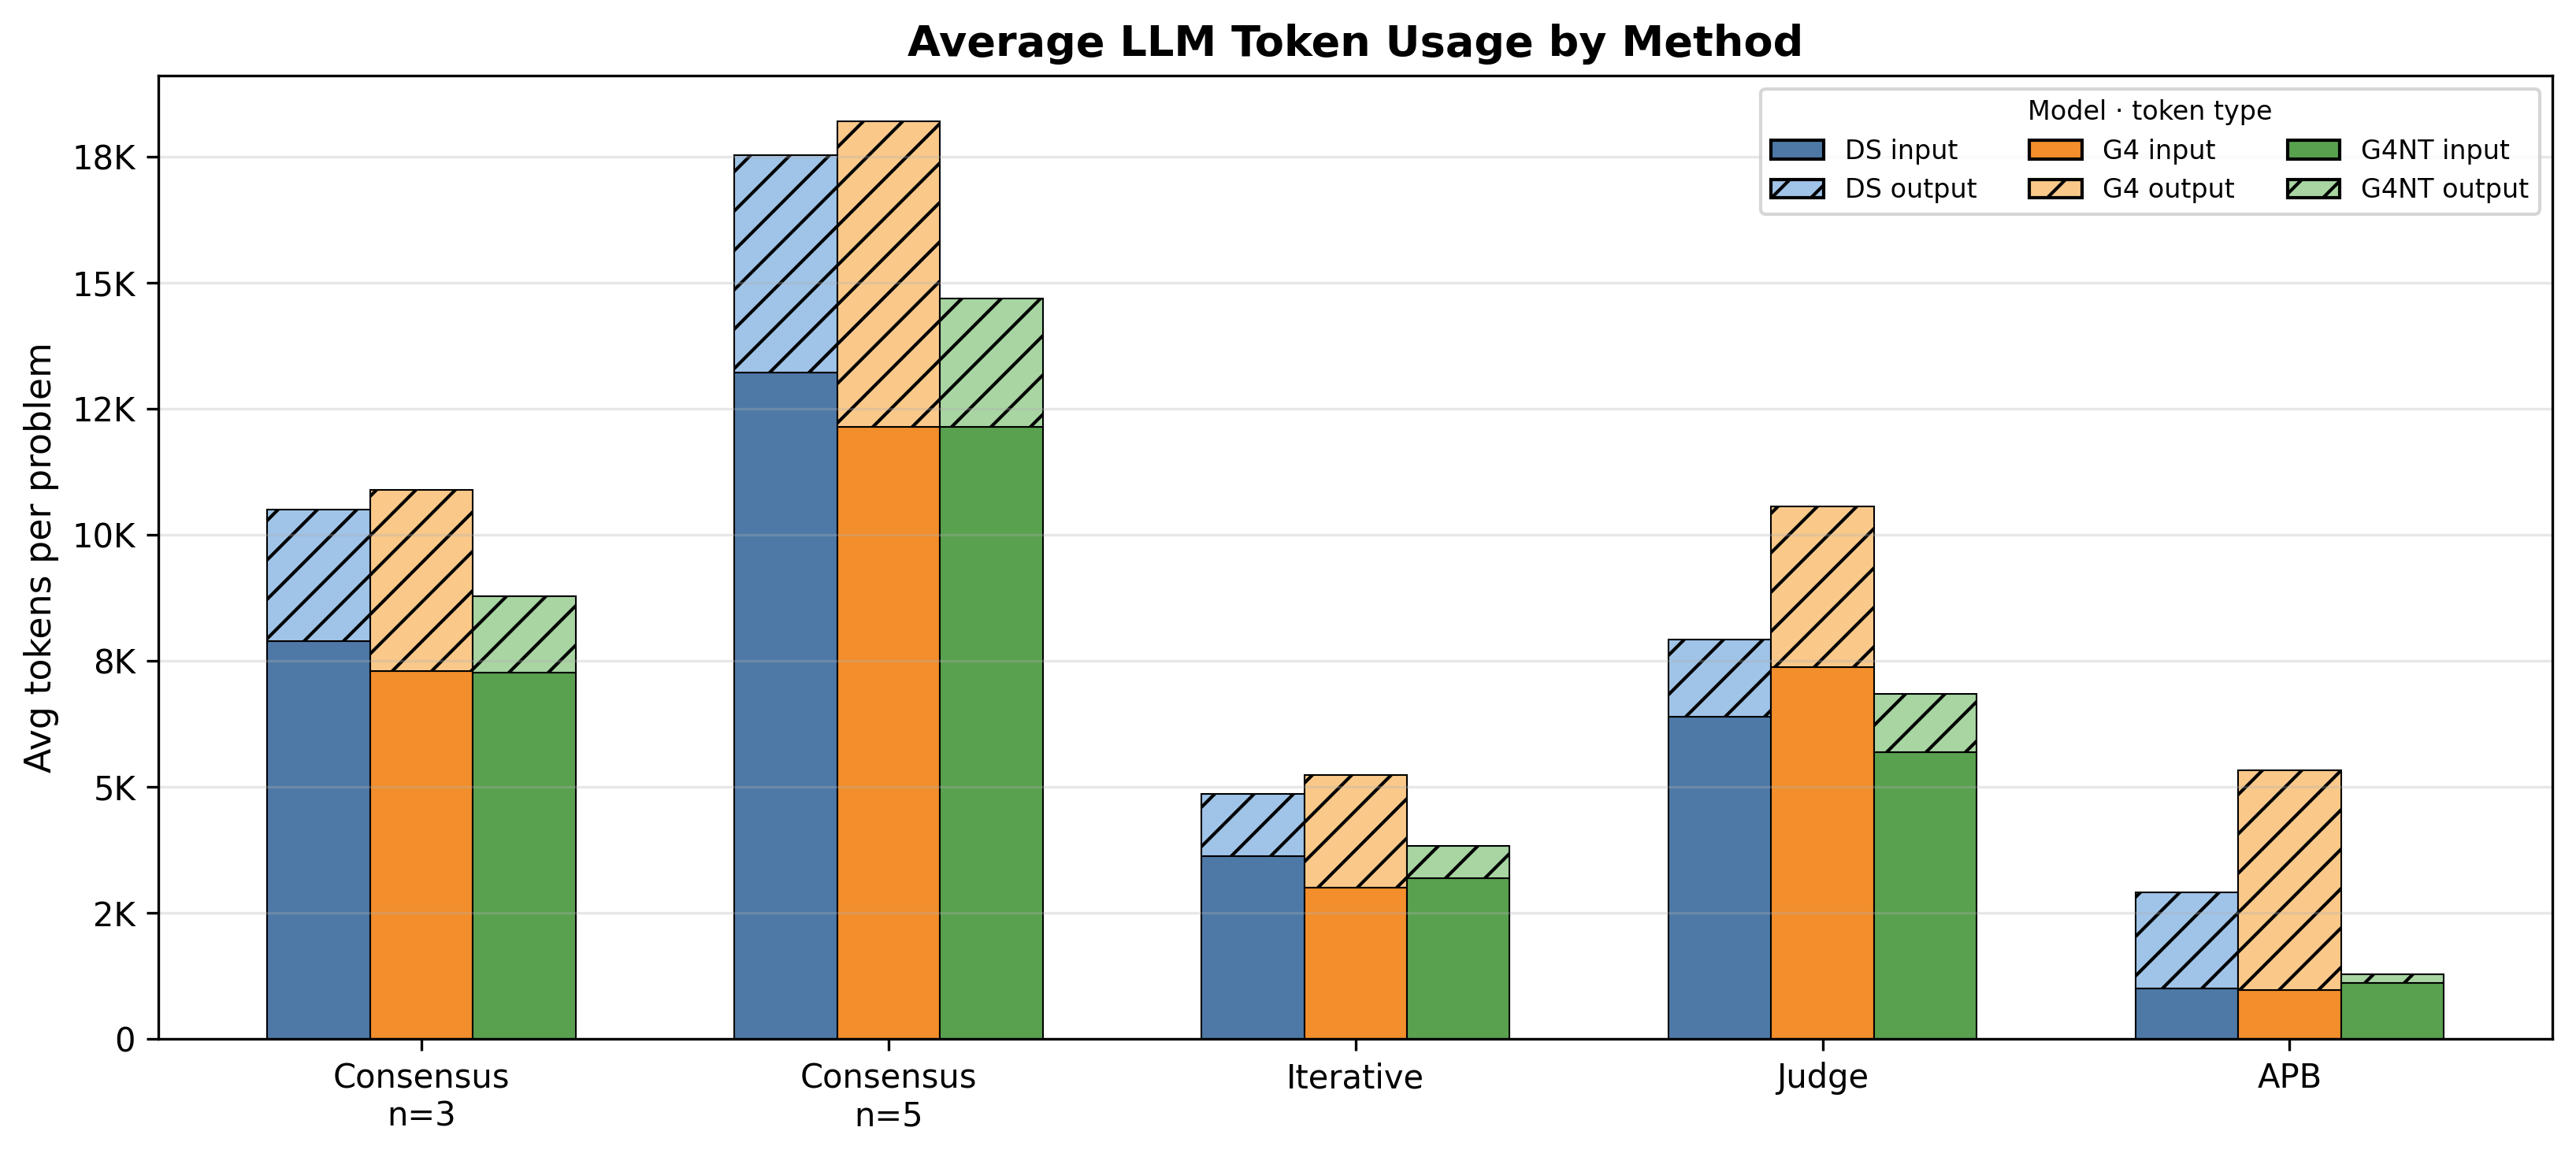
\includegraphics[width=0.45\textwidth]{figures/token_usage.png}
  \caption{\small{Average LLM token usage per problem (input: solid, output: hatched) across methods and models. Error bars show $\pm 1$ standard deviation of the total tokens per problem.}}
    \label{fig:token_usage}
\end{figure}

\section{Conclusion \& Future Work}

% We have shown that small, single-GPU open-weight LLMs, used across three CAST variants, can both recover valid plans for unsolvable problems and appropriately refuse when no valid substitution exists, substantially outperforming both LLM-based baselines across problem categories and semantic encodings. 

We introduced CAST, a neuro-symbolic component that operates upstream of a symbolic planner. CAST repairs runtime typing gaps by revising only the object-to-type assignments, making a minimal and constrained alteration to the symbolic knowledge used for planning.
Through our experiments, we show that CAST generally outperforms unconstrained PDDL repair and end-to-end LLM planning across substitution problems, distractor settings, and semantically varied domains. Our results also reveal a recovery--refusal trade-off: iterative refinement provides strong recovery at low token cost, whereas judge-based selection more reliably rejects invalid substitutions. A physical-robot demonstration further shows that CAST can be integrated into an open-vocabulary perception--planning--action pipeline.

Our approach has limitations that warrant further investigation. CAST offers no formal guarantees that substitutions made are valid. A \texttt{pick-up} action, for instance, may only apply to rigid objects and may not transfer to deformable ones. An avenue for future work can involve active probing for affordance discovery at runtime, enabling agents to test if actions can be successfully applied to an object before updating the symbolic representation. Additionally, we rely on the action name being semantically rich enough to describe its use; a less descriptive encoding like \texttt{action1} would give the LLM no signal about the affordances of \texttt{pickup-object} or which objects it applies to. Encoding affordances alongside actions, rather than relying on the action name alone, could give the LLM a more reliable signal for judging functional fit. 
